\section{Softwarearchitektur}

Im Bereich der Softwarearchitektur wurde die zentrale Verarbeitungskette für die sprachliche Interaktion aufgebaut.
Ziel war es, eine durchgängig lauffähige Systemkette zu entwickeln, in der eine gesprochene Anfrage vollständig erfasst, verarbeitet und beantwortet werden kann.

\subsection{Ergebnis}

Die Softwarearchitektur von Pablo basiert auf einer modularen, ereignisgesteuerten Python-Struktur mit Trennung zwischen Ein- und Ausgabe, Dialogverarbeitung sowie Hardwaresteuerung. 
Beim Start werden zunächst die Systemkonfiguration, die verfügbaren Plugin-Module und die visuelle Prozessdarstellung initialisiert. 
Anschließend wird der Wakeword- und Richtungsdetektor konfiguriert, der als Trigger-Komponente für die Interaktionsschleife fungiert.
Die aus der Wakeword-Analyse abgeleitete Schallrichtung wird unmittelbar auf die Servosteuerung übertragen, sodass sich der Bildschirm in Richtung der sprechenden Person ausrichtet.

Das System durchläuft eine Hauptschleife in vier funktional entkoppelten Phasen:

\textbf{(1) Aktivierung des Systems}

Die Aktivierung erfolgt über eine Wakeword-Erkennung mit Picovoice Porcupine. 
Beim Erkennen des Wakewords wird zeitgleich die Schallrichtung aus einem gepufferten Stereo-Audiofenster mittels GCC-PHAT-Korrelation der beiden Mikrofonkanäle bestimmt und zur Servo-Ausrichtung genutzt. 
Die Servosteuerung erfolgt asynchron in einem separaten Thread, sodass die Audioverarbeitung nicht blockiert wird. 

\textbf{(2) Spracherkennung (STT)}

Die Spracherkennung erfolgt mit dem Vosk-Framework. 
Der Audiostrom wird verarbeitet, bis das Vosk-Modell einen vollständigen Satz erkannt hat. 
Erst dann wird der Text an die Dialogverarbeitung übergeben.

\textbf{(3) LLM-Verarbeitung}

Die inhaltliche Verarbeitung nutzt eine API für den Zugriff auf ein Large-Language-Model (Llama 3.3 70B). 
Der erkannte Nutzereingabe-Text wird zusammen mit den vom Plugin-Loader geladenen Tool-Definitionen an das Modell übergeben. 
Durch den bereitgestellten Kontext kann das System zwischen generischer Antwortgenerierung und Modulausführung unterscheiden. 
Das Modell entscheidet selbstständig, ob ein direkter Chat-Response ausreicht oder ob ein registriertes Plugin-Tool aufgerufen werden soll. 
Die Plugins kapseln die Logik für Wetter, Notizen, Kalender und Timer.

\textbf{(4) Sprachausgabe (TTS)}

Die Sprachausgabe wird lokal mit Piper generiert (deutsches Modell \texttt{de\_DE-thorsten-low.onnx}). 
Der Text wird in eine WAV-Datei gerendert und über einen System-Audio-Player abgespielt. 
Vor dem eigentlichen Audiomaterial wird eine führende Stille eingefügt, sodass die visuelle Feedback-Umschaltung mit dem tatsächlichen Audiobeginn zeitlich synchronisiert ist.

\begin{figure*}[htbp]
	\centering
	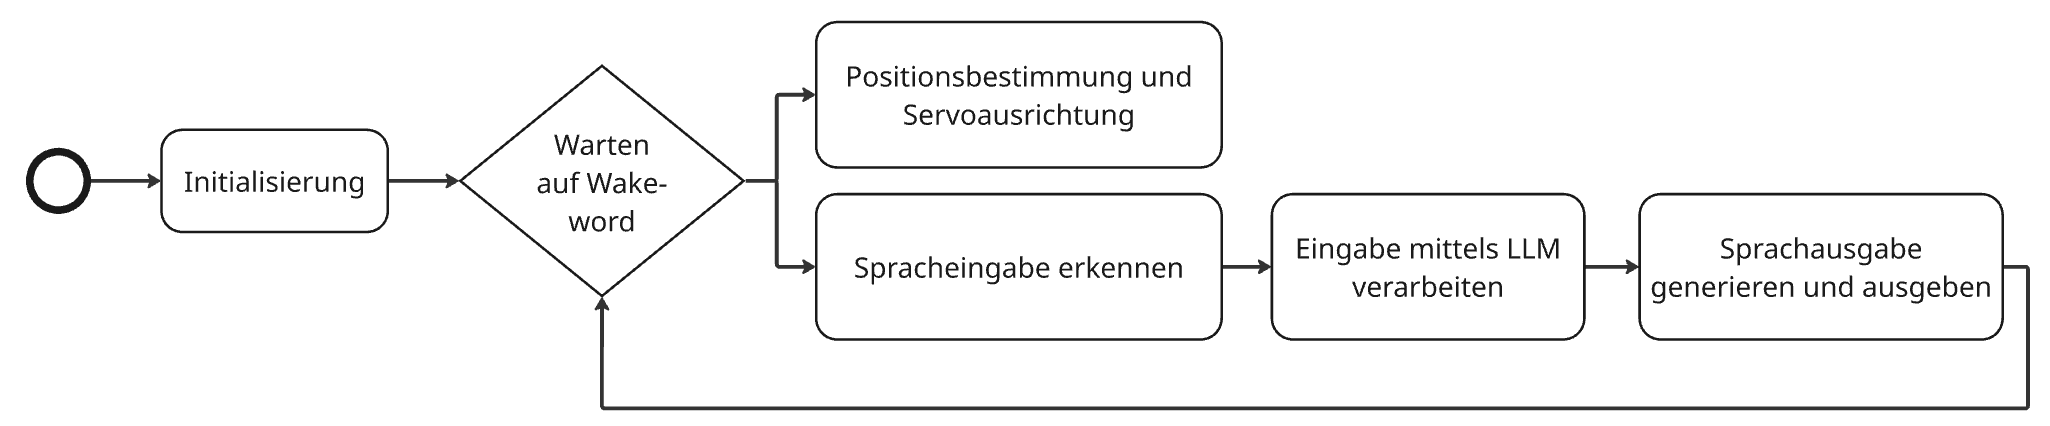
\includegraphics[width=0.75\textwidth]{grafiken/Hauptschleife.png}
	\caption{Ablauf der Hauptschleife von Pablo.}
	\label{fig:hauptschleife}
\end{figure*}

Die einzelnen Phasen sind funktional entkoppelt und über definierte Funktionsaufrufe miteinander verbunden.
Fehlerfälle werden über Ausnahmebehandlung auf Schleifenebene abgefangen. 


\subsection{Einordnung}

Die Softwarearchitektur wurde auf Modularität und Austauschbarkeit ausgelegt. 
Durch die funktionale Trennung von Aktivierung, Spracherkennung, LLM-Verarbeitung, Modulausführung, Sprachausgabe und Hardwareansteuerung konnte die Komplexität des Gesamtsystems reduziert werden. 
Gleichzeitig lassen sich einzelne Komponenten, etwa für STT, TTS oder das Sprachmodell, ersetzen, ohne den gesamten Ablauf grundlegend anzupassen.

Eine zentrale Entwicklungsentscheidung war die Kopplung der Plugin-Schnittstelle an die LLM-Verarbeitung. 
Dadurch kann das System zwischen freier Antwortgenerierung und gezieltem Funktionsaufruf unterscheiden, ohne dass für jeden Anwendungsfall feste Entscheidungslogiken im Quellcode hinterlegt werden müssen. 
Dies ermöglicht eine flexiblere Verarbeitung natürlicher Sprache und unterstützt eine weniger schematische Interaktion.

Auch die Auswahl des Sprachmodells erfolgte iterativ. 
Hierfür wurden mehrere Modelle hinsichtlich ihrer Fähigkeit verglichen, den bereitgestellten Systemkontext zu verarbeiten und inhaltlich sinnvolle Antworten zu erzeugen. 
Das gewählte Modell zeigte dabei die geeignetste Verarbeitung des Kontexts im bestehenden Anwendungsszenario. 
Aufgrund der modularen Architektur bleibt jedoch auch das LLM grundsätzlich austauschbar, sodass dieses auf andere Anwendungsfälle angepasst werden kann.

Für die Aktivierung wurde eine wakeword-basierte Lösung umgesetzt, um einen durchgängig sprachlichen und freihändigen Zugang zum System zu ermöglichen. 
Vosk wurde für die Spracherkennung gewählt, da es lokal ausführbar ist und sich gut in die Python-basierte Systemumgebung integrieren lässt. 
Für die Sprachausgabe wurde mit Piper ebenfalls eine lokal ausführbare Lösung verwendet, sodass zentrale Teile der Sprachpipeline ohne zusätzliche externe Dienste umgesetzt werden konnten.

Die asynchrone Ausführung von Servoansteuerung und visuellen Zustandswechseln wurde gewählt, um blockierende Abläufe von der Sprachverarbeitung zu entkoppeln. 
Dadurch bleibt die Reaktionsfähigkeit des Systems auch bei parallel ablaufenden Teilprozessen erhalten.

Insgesamt ist die Softwarearchitektur auf Erweiterbarkeit, Integrationsfähigkeit und einen stabilen interaktiven Ablauf ausgelegt und bildet damit eine geeignete Grundlage für die prototypische Umsetzung von Pablo.